\section{Opis ogólny}

\subsection{Perspektywa produktu}
System SWPFK ma na celu zastąpienie istniejącego systemu, który jest już przestarzały oraz nie spełnia wymagań firmy kurierskiej. Będzie on funkcjonował jako niezależne oprogramowanie wspomagające szereg procesów związanych z usługami dostarczanymi przez firmę.

System będzie udostępniał \textbf{klientom firmy} interfejs za pomocą, którego będą mogli zamówić odpowiednie usługi oraz uzyskać niezbędne informacje. Interfejs ten powinien być oparty na technologii zapewniającej szeroką dostępność dla klientów firmy.

\textbf{Kurierom} system będzie dostarczał mobilnego rozwiązania wspomagającego proces odbioru i doręczenia przesyłek. Rozwiązanie to będzie zbudowane w oparciu o urządzenia mobilne zapewniające bezprzewodową łączność z systemem.

\textbf{Pracownikom obsługi klienta} system będzie dawał możliwość dostępu do pełnej historii klienta i informacji o nim. Istotne jest aby wykorzystany interfejs zapewniał wysoką przejrzystość prezentowanych danych.

\textbf{Pracownicy sortowni} będą mieli dostęp do interfejsów zapewniających im pomoc w odpowiednim uszeregowaniu przesyłek oraz zaplanowaniu trasy doręczenia aby zmaksymalizować efektywność tych procesów. Wspomniany interfejs powinien zapewniać wysoką wydajność oraz przyjazną wizualizację wyników algorytmu.

System będzie również udostępniał interfejsy umożliwiające integrację z \textbf{systemami zewnętrznych firm} transportowych w celu korzystania z ich usług z poziomu SWPFK.

Rysunek \ref{diag:perspektywa} przedstawia diagram kontekstu dla SWPFK. Zawiera on podstawowych aktorów prowadzących interakcję z systemem oraz podstawowe informacje jakie będą z~nim wymieniać.

\begin{figure}[ht]
	\centering
	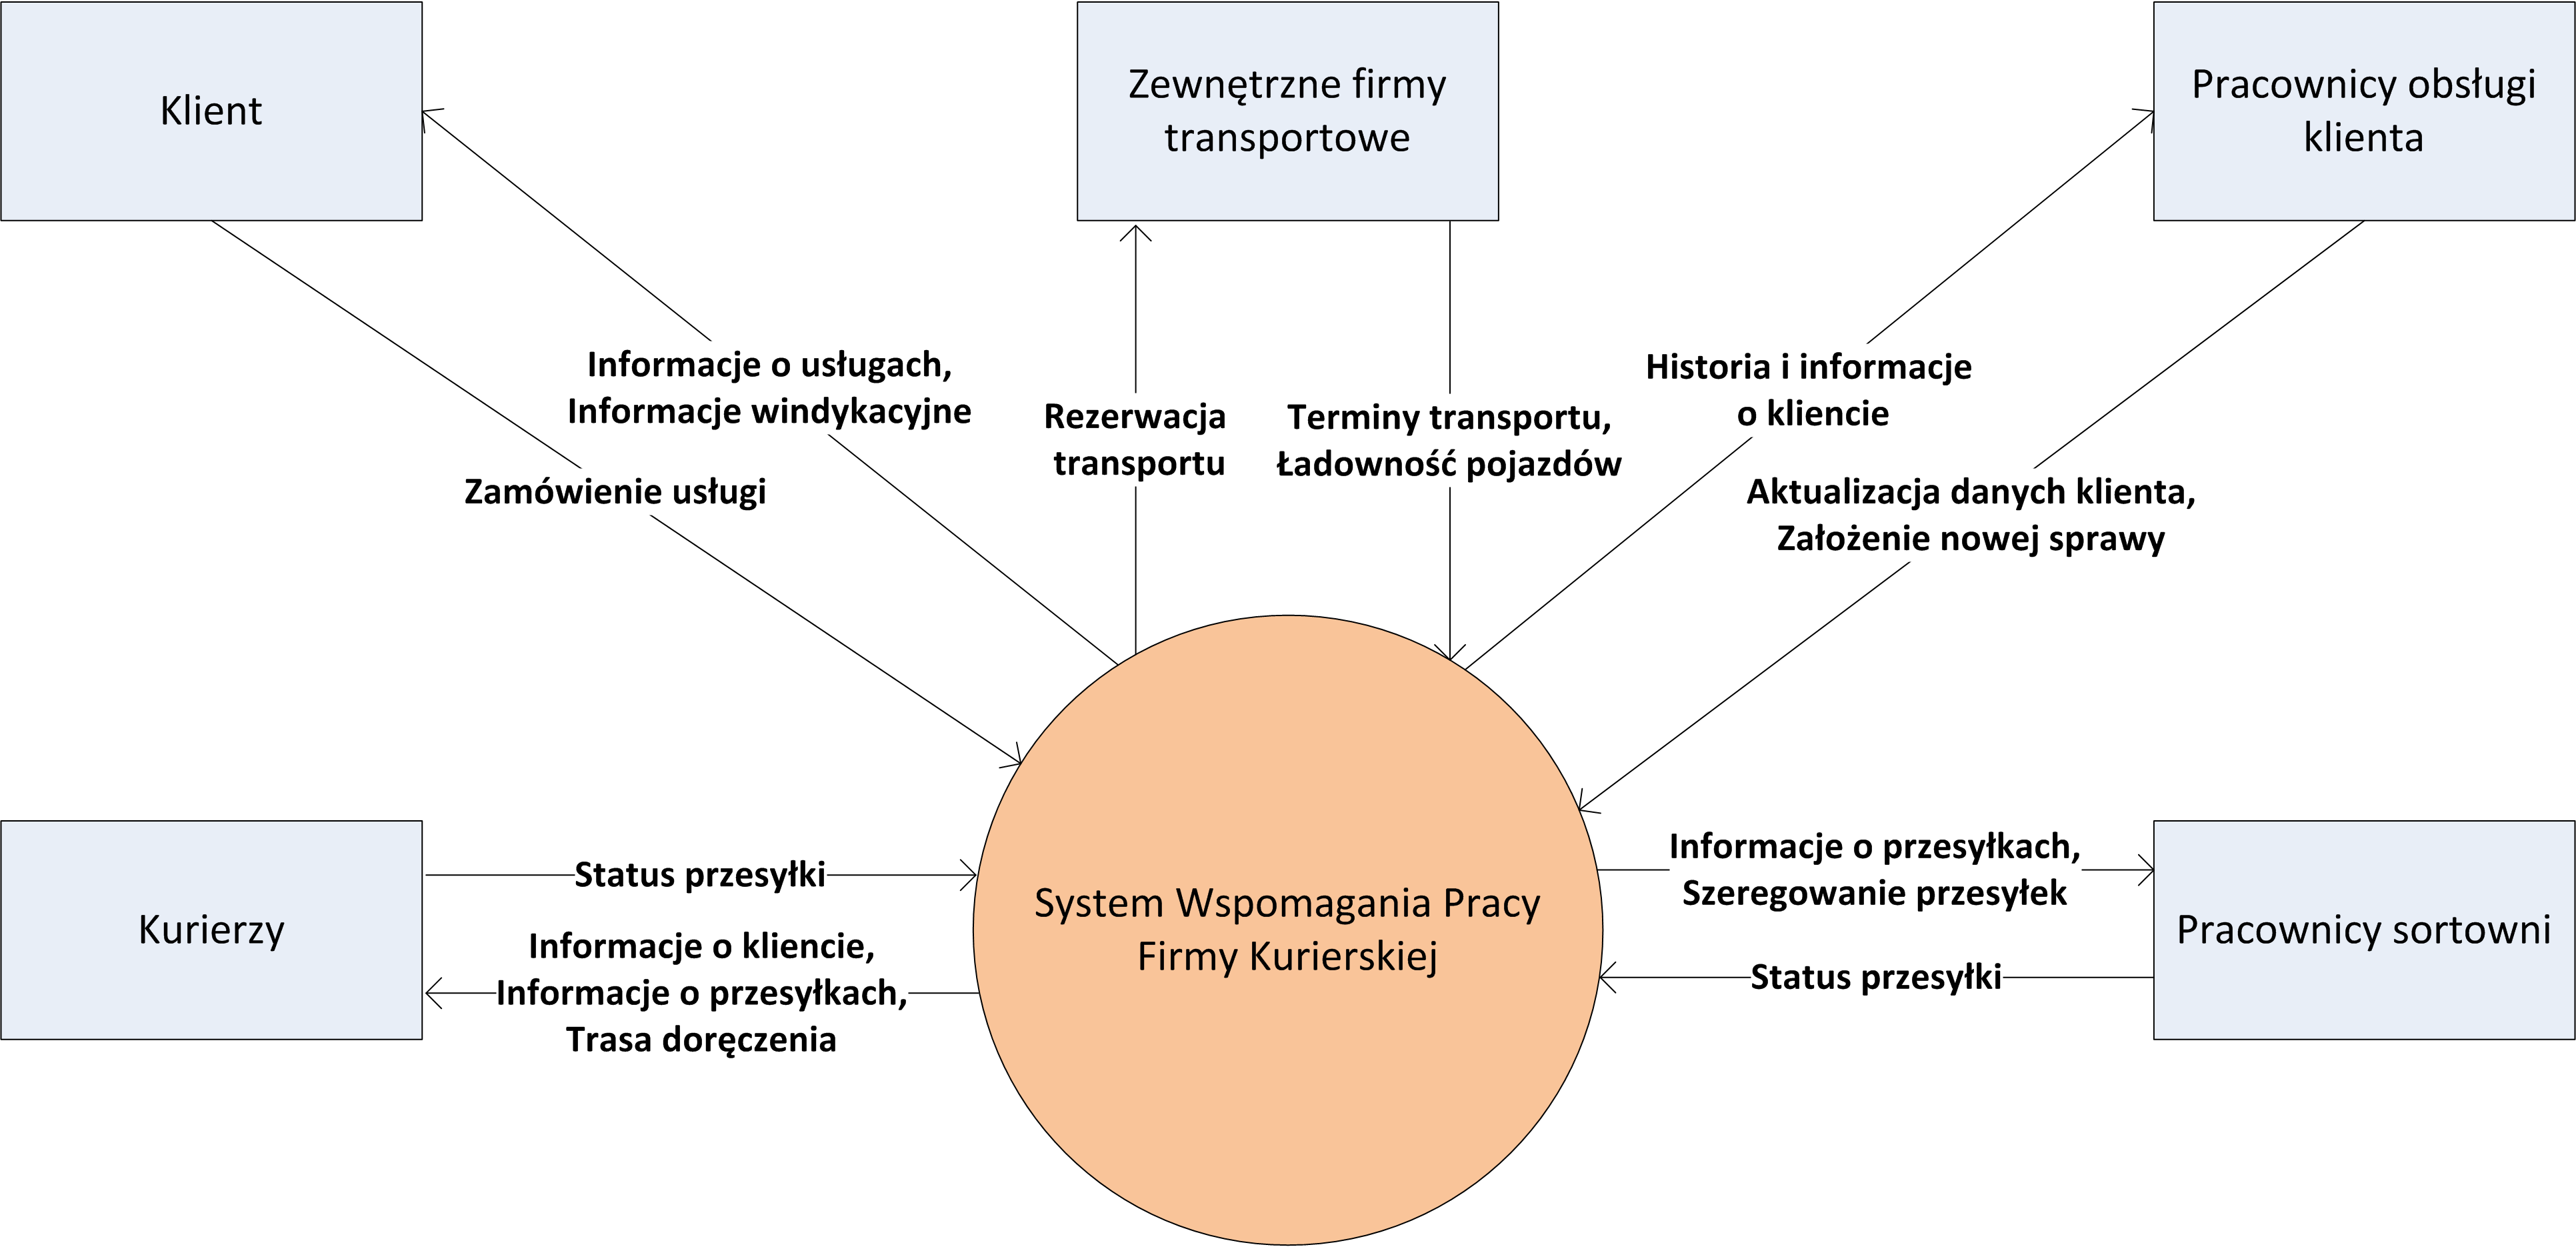
\includegraphics[width=\textwidth]{img/perspektywa}
	\caption{Diagram kontekstu dla SWPFK.}
	\label{diag:perspektywa}
\end{figure}

\subsection{Funkcje produktu}
Podstawową funkcją SWPFK będzie możliwość rejestracji przesyłki w systemie oraz śledzenie jej drogi od momentu nadania do doręczenia. Ponadto pozwoli on na odpowiednie zoptymalizowanie transportu przesyłek oraz wyznaczenie najlepszej drogi ich doręczenia do adresata.

System będzie zapewniał klientom firmy kurierskiej możliwość stałego dostępu do szczegółowych informacji na temat usług świadczonych przez firmę. SWPFK będzie również udostępniał możliwość zamówienia dowolnej usługi za pomocą odpowiednich interfejsów, skorzystania z pomocy obsługi klienta oraz rejestracji klienta w systemie.

Pracownicy obsługi klienta będą używać SWPFK w celu:
\begin{itemize}
\item obsługi klientów w POK;
\item dostępu do przekrojowej informacji o kliencie, która będzie zawierała m. in. jego pełną historię;
\item obsługi klientów kanałem online.
\end{itemize}

System będzie również umożliwiał zamówienie usługi transportu w zewnętrznej firmie transportowej oraz obsługę windykacji w szczególności klientów masowych.

\subsection{Ograniczenia}

\subsubsection{Zgodność z aktami prawnymi}
SWPFK musi być zgodny z rozporządzeniami oraz ustawami wymieniowymi w rozdziale \ref{subsec:Literatura} w punktach 1, 2 oraz 3.

\subsubsection{Zgodność ze standardami i normami}
Dokumentacja użytkownika musi być zgodna ze standardem IEEE 1063-2001 (punkt 4 w rozdziale \ref{subsec:Literatura}).

\subsubsection{System zarządzania bazą danych}
Firma Kurierska posiada 4 licencje na bazę danych firmy Oracle w wersji 10g z możliwością aktualizacji do wersji 11g. Licencje są w wersji Enterprise Edition oraz typu procesorowego co pozwala na użytkowanie bazy przez wielu użytkowników. Do licencji zostało również wykupione wsparcie na wypadek wystąpienia problemów w obsłudze bazy danych.

Ze względu na posiadane licencje SWPFK powinien być zbudowany w oparciu o bazę danych firmy Oracle. SWPFK będzie agregował duże ilości danych dotychczas rozproszonych po odseparowanych systemach co może skutkować koniecznością dokupienia większej ilości licencji, aby móc zainstalować system na sprzęcie o większej mocy obliczeniowej.

Wykorzystanie posiadanych licencji pozwoli na obniżenie kosztów systemu oraz zaangażowanie dotychczas zdobytego doświadczenia w obsłudze baz danych Oracle.

\subsubsection{Ograniczenia sprzętowe}
\subsubsection*{Infrastruktura sieciowa}
Moduł serwerowy SWPFK będzie uruchomiony w jednej fizycznej lokalizacji. Z tego względu wymaga się, aby serwerownia w której będzie uruchomiony moduł serwerowy SWPFK miała zapewnione co najmniej dwa redundantne połączenia światłowodowe do sieci Internet. Każde z tych połączeń powinno pochodzić od innego ISP oraz charakteryzować się przepustowością na poziomie co najmniej 10 Gb/s. Ponadto każde z połączeń musi zapewniać dostępność na poziomie minimum 99,999\% w~skali miesiąca.

Ponadto połączenia sieciowe między dowolnymi dwoma elementami serwerowni powinny charakteryzować się przepustowością co najmniej 10 Gb/s.

\subsubsection*{Konfiguracja sprzętowa serwera}
Wymaga się aby moduł serwerowy SWPFK był w stanie obsłużyć jednocześnie  do 10000 równoległych sesji użytkowników korzystających z interfejsu internetowego oraz prowadzić obsługę innych aplikacji SWPFK spełniając wszystkie stawiane przed SWPFK wymagania wydajnościowe. 

W celu spełnienia wymagań niezawodności SWPFK powinien być uruchomiony na dwóch niezależnych serwerach, z których jeden będzie pełnił funkcję zapasową i przejmie obsługę SWPFK tylko w sytuacji awarii głównej instancji.

W poniższej tabeli znajduje się minimalna konfiguracja serwera obsługującego moduł serwerowy SWPFK.

\begin{center}
\begin{tabular}[h]{|p{3.5cm}|p{11.6cm}|}
\hline
Procesory: & 16 procesorów 12-wątkowych o częstotliwości taktowania zegara 2,5 GHz i 15 MB pamięci podręcznej, np. Intel E5-2630 v2 lub inny o nie niższej mocy obliczeniowej\\ \hline
Pamięć RAM: & 512 GB \\ \hline
Karta sieciowa: & Dwie karty sieciowe każda o przepustowości 10 Gb/s \\ \hline
Pojemność dyskowa & Efektywnie 10 TB, dyski działające w macierzy typu RAID 5 \\ \hline
System operacyjny: & SUSE Linux Enterprise Server 11 \\ \hline
Dodatkowe oprogramowanie: & Java w wersji co najmniej 1.7 \\
\hline
\end{tabular}
\end{center}

\subsubsection*{Stacja robocza dla aplikacji klienckiej}
Minimalne wymagania aplikacji klienckiej SWPFK do poprawnego działania na stacji roboczej przedstawia poniższa tabela.

\begin{center}
\begin{tabular}[h]{|p{3.5cm}|p{11.6cm}|}
\hline
Procesor: & Intel Core i3 1,8 GHz lub inny o zbliżonej mocy obliczeniowej \\ \hline
Pamięć RAM: & 1,5 GB \\ \hline
Karta sieciowa: & 100Mb/s \\ \hline
Dostępna pojemność dysku: & 1,5 GB \\ \hline
System operacyjny: & Windows Vista \\ \hline
Dodatkowe oprogramowanie: & Microsoft .NET Framework 3.5 \\
\hline
\end{tabular}
\end{center}

\subsubsection{Protokoły komunikacyjne}
SWPFK powinien wykorzystywać w komunikacji jedynie otwarte protokoły komunikacyjne sieci Internet.

\subsubsection{Instalacja oprogramowania}
Aplikacja kliencka instalowana na komputerach PC nie powinna wymagać praw administratora aby zostać zainstalowana. Ponadto instalator aplikacji klienckiej powinien być dystrybuowany w postaci pojedynczego, niezależnego pliku. Plik ten po uruchomieniu powinien przeprowadzić użytkownika przez proces instalacji w formie czytelnego kreatora. Zakłada się, że do instalacji użytkownik nie będzie potrzebował żadnej specjalistycznej wiedzy z zakresu obsługi komputerów.

Aplikacja mobilna będzie instalowana na terminalach mobilnych przez wyspecjalizowanych techników. Również moduł serwerowy będzie instalowany na serwerze przez osoby posiadające zaawansowaną wiedzę z zakresu utrzymywania i instalacji oprogramowania serwerowego.

\subsubsection{Interfejsy programistyczne}
Wszystkie moduły SWPFK powinny implementować interfejsy programistyczne tak aby były one możliwe do osiągnięcia za pomocą technologii Java oraz .NET Framework bez ponoszenia kosztów implementacji własnych bibliotek obsługujących niestandardowe rozwiązanie.

\subsection{Dokumentacja użytkownika}
Dokumentacja SWPFK będzie się składać z:
\begin{center}
\begin{tabular}[h]{|p{2cm}|p{13.1cm}|}
\hline
Nazwa: & Dokumentacja techniczna SWPFK \\ \hline
Opis: & Dokument będzie opisywał architekturę wszystkich modułów SWPFK, zastosowane technologie i rozwiązania oraz instrukcje instalacji i utrzymania każdego modułu. \\ \hline
Standard: & IEEE 1063-2001 \\ \hline
Format: & elektroniczny (w formie pliku PDF), drukowany \\ \hline
Język: & angielski \\
\hline
\end{tabular}
\end{center}

\begin{center}
\begin{tabular}[h]{|p{2cm}|p{13.1cm}|}
\hline
Nazwa: & Przewodnik użytkownika aplikacji klienckiej \\ \hline
Opis: & Dokument będzie zawierał szczegółowy opis wszystkich dostępnych  funkcjonalności aplikacji klienckiej. Będzie również zawierał opis każdego okna aplikacji. \\ \hline
Standard: & IEEE 1063-2001 \\ \hline
Format: & elektroniczny (w formie pliku PDF), drukowany \\ \hline
Język: & polski, angielski, niemiecki, hiszpański, francuski, czeski, słowacki \\
\hline
\end{tabular}
\end{center}

\begin{center}
\begin{tabular}[h]{|p{2cm}|p{13.1cm}|}
\hline
Nazwa: & Przewodnik użytkownika aplikacji mobilnej \\ \hline
Opis: & Dokument będzie zawierał szczegółowy opis wszystkich dostępnych  funkcjonalności aplikacji mobilnej oraz sposób ich użycia.  \\ \hline
Standard: & IEEE 1063-2001 \\ \hline
Format: & elektroniczny (w formie pliku PDF), drukowany \\ \hline
Język: & polski, angielski, niemiecki, hiszpański, francuski, czeski, słowacki \\
\hline
\end{tabular}
\end{center}

\subsection{Założenia i zależności}
Zakłada się, że użytkownik interfejsu internetowego SWPFK będzie korzystał z jednej z poniższych przeglądarek internetowych:
\begin{enumerate}
\item Internet Explorer 10, 11;
\item Mozilla Firefox w wersji co najmniej 28;
\item Google Chrome w wersji 35 lub wyższej;
\item Apple Safari w wersji co najmniej 5.
\end{enumerate}

Zakłada się, że użytkownicy aplikacji klienckiej na komputer PC będą korzystać z systemu Microsoft Windows Vista lub jego nowszej wersji. Ponadto użytkownicy będą mieli zainstalowane oprogramowanie Microsoft .NET Framework w wersji co najmniej 3.5.